\section{基本概念}
以下三种关系是C++中常见的,读者务必搞清楚它们之间的区别,切勿混淆。\par
\subsection*{整体与部分(Has-a relationship)}
还记得我们在第六章讲述结构体时如何说吗?
\begin{lstlisting}
    int cuboid[3]; //定义一个3长度数组,用来表示一个长方体
\end{lstlisting}
通过这种方式,我们定义了一个数组用以表示长方体,但它终究是三个孤立的值(只是存放在一起方便访问),而不是一个``整体''——比如说,函数的返回值只能是单个数据,而不能是数组。这就好比,我们已经有了发动机、轮胎、蓄电池、保险杠等等一应俱全的零件,但就是没有一辆完整的汽车。\par
所以我们应该把这样一盘散沙的零件封装成一个完整的对象,这样也就有了``整体与部分''的概念。\par
一辆汽车,它的发动机就是它的一部分;一个人,他的大脑和心脏就是他的一部分;一个动物园,它的各个展区——狮子区、老虎区等,都是它的一部分;一个国家,它的各个城市,都是它的一部分。\par
以上所述,都是\textbf{``整体与部分''的关系,用英文可以阐述为``Has-a relationship'',在C++中可以诠释为``对象与成员''}。如果我们定义一个 \lstinline@valarri@ 类的 \lstinline@a@,那么 \lstinline@a@ 就是对象,\lstinline@a._size@, \lstinline@a._cap@ 和 \lstinline@a._arr@ 都是成员。这些成员如果单独存在,它表达的含义就不明显了;但是倘若它们存放在一起,那么我们就可以根据它们各自的值,以及它们之间的相互关系,从而表示更丰富、更明确的含义。\par
我们在第八章曾讲过,一个类的成员同时也是另一个类的对象——这说明整体与部分的关系是有传递性的。作为汽车一部分的发动机,它也是由气缸、活塞、燃油泵等部分构成的。就这样,我们可以把一个对象拆解成若干成员,又把这些作为成员的对象拆解成更小单位的成员,一直拆解到 \lstinline@int@, \lstinline@double@ 等基本类型及它们的指针、数组类型。\par
\subsection*{模板与实例}
我们曾在第四章简单地讲解过泛型编程的概念。我们说,泛型编程并不直接定义具体的函数,而是定义了一个模板(Template)。
\begin{lstlisting}
template<typename T>
T user::max(const T& lhs, const T& rhs) {
    return lhs > rhs ? lhs : rhs;
}
\end{lstlisting}
如果我们在代码中需要调用它来进行两个 \lstinline@double@ 数据求最大值,那么编译器就会照此模板生成一个 \lstinline@user::max(const double&,const double)@ 函数,我们把它称为这个模板的实例(Instance)。一个模板可能有千奇百怪的实例,用以处理各种不同的数据,但它们总有很多的相似之处。\par
现在我们把``模板与实例''这个概念扩展到更广义的层面上去。模板就是一个抽象的概念,它不对应着什么实体;而实例正是在这个模板概念之下产生的实体。``人类''就是这样的一个模板,它只是一个抽象概念,不对应任何实体;而``张三''``李四''这样的实体就是这个模板的实例,他们可能有不同的属性,比如身高、体重,但总有一些独特的、能与其它物种分开的属性,比如``读写能力''之类的。\par
这种\textbf{``模板与实例''的关系,用英文可以阐述为``Instance-of relationship'',在C++中可以诠释为``类与对象''}。对于我们定义的 \lstinline@valarri a@ 来说,\lstinline@valarri@ 就是类,而 \lstinline@a@ 就是对象。\par
初学者很容易搞混``Instance-of relationship''与``Has-a relationship'',但只要记住一点:``类''是一个抽象的概念,不对应实体;而``对象''和``成员''都是具体的事物,它们对应着实体\footnote{这不是金科玉律!但是对于日常生活中九成以上的情况来说都足够了。}。也正因为``类''与``对象''不是同一层次的概念,所以``模板与实例''的关系是没有传递性的。\par
\subsection*{属与种}
在讲述这个关系前我想请读者思考一个问题:我家的哈士奇和李四家的萨摩耶是同类吗?\par
是吗?好像不是。不是吗?好像也是。\par
之所以存在这样的困惑,是因为我们没说清``同类''是什么概念。对于我家的哈士奇来说,它属于``哈士奇类(Husky)'';而对于李四家的萨摩耶来说,它属于``萨摩耶类(Samoyed)''——那么它们当然不是同类了。\par
但是我们还有另一种观察角度:无论我家的哈士奇还是李四家的萨摩耶,它们都属于``家犬亚种(Canis lupus familiaris)''——那么它们当然是同类了。\par
这时你就会发现一个问题:好像我家的哈士奇同时属于``家犬''和``哈士奇''哎。其实不只如此,它还属于``狼种(Canis lupus)''``犬属(Canis)''``犬科(Canidae)''``食肉目(Carnivora)''``	哺乳纲(Mammalia)''``脊索动物门(Chordata)''``动物界(Animalia)''。看上去是不是很复杂?很吓人?\par
问题来了。在我们既有的认知中,一个对象只能是单个类的对象,那么现在它同时是这么多类的对象,这岂不是乱套了?其实并不会,因为这些类之间存在着一种\textbf{``属与种''的关系。用英文可以阐述为``Is-a relationship'',在C++中可以诠释为``基类与派生类''。\footnote{值得一提的是,一般我们只用公开继承/受保护继承来表示``Is-a relationship'';至于私有继承,它更适合用来表示``Has-a relationship''。}}\par
``属与种''的关系描述的是两个类的关系,它们有点像数学上的集合间包含关系——如果一个对象是类 \lstinline@A@ 的对象,那么它一定也是类 \lstinline@B@ 的对象。在这个关系当中,\lstinline@A@ 就是基类,而 \lstinline@B@ 是派生类。对于派生类的对象来说,它既有基类的共性——比如我家哈士奇能``汪汪''叫,王五家的泰迪也能,又有派生类的独特性——比如我家哈士奇是拆家小能手,但王五家的泰迪就不能胜任了。\par
\subsection*{何为继承?}
\textbf{继承(Inheritance)}是一种代码重用的好方法。如果我们已经写了一个类 \lstinline@Dog@,而我们想要再写一个 \lstinline@Husky@ 类,那么我们没必要把 \lstinline@Dog@ 已有的那部分功能再写一遍,直接让 \lstinline@Husky@ 类继承 \lstinline@Dog@ 类就足够了——然后我们只需要集中精力去写诸如``拆家''之类的独特功能即可。\par
\begin{lstlisting}
struct Dog { //狗类
    unsigned age; //所有的狗都有年龄属性
    double weight; //所有的狗都有体重属性
    //...
};
struct Husky : Dog { //哈士奇类,公开继承自狗类
    void destroy() { /*...*/ } //哈士奇独特的拆家本领
};
int main() {
    Husky mine {5, 27}; //哈士奇类的对象拥有狗类的成员
    std::cout << mine.age << ' '; //输出mine的年龄
    std::cout << mine.weight; //输出mine的体重
    mine.destroy(); //拆家,开始执行
}
\end{lstlisting}
在这个继承操作当中,\lstinline@Husky@ 类继承自 \lstinline@Dog@ 类。其中的 \lstinline@Husky@ 称为\textbf{派生类(Derived class)},而 \lstinline@Dog@ 称为\textbf{基类(Base class)}。派生类的对象拥有基类的成员,所以 \lstinline@mine@ 可以使用 \lstinline@age@, \lstinline@weight@ 等基类成员,就好像它们定义在了 \lstinline@Husky@ 类当中一样,如图所示。
\begin{figure}[htbp]
    \centering
    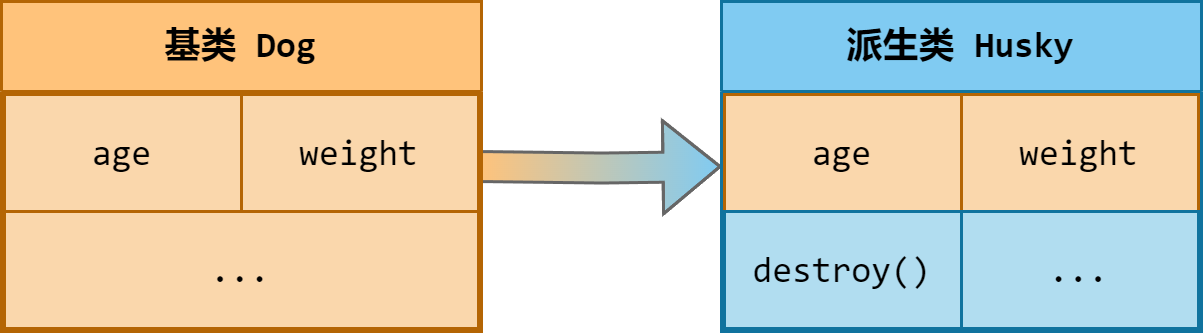
\includegraphics[width=.8\textwidth]{../images/generalized_parts/09_dog_and_husky_relationship_300.png}
    \caption{\lstinline@Dog@ 类的成员与 \lstinline@Husky@ 类的成员}
\end{figure}\par
